\chapter{THE STANDARD MODEL OF PARTICLE PHYSICS}
\label{ch:theory}
The Standard Model (SM) is a collection of the most accurate and self-consistent particle physics theories that mathematically describe the properties of particles within the Universe and their interactions with each other~\cite{Glashow:1961tr,PhysRevLett.19.1264}.
For the past century, some of the most brilliant minds in physics have spent their entire careers to develop equations, mathematical tricks, and completely novel ideas to help build a solid foundation for the SM.

To demonstrate the unparalleled accuracy with which the SM predicts physical phenomena, one needs to look no further than the anomalous magnetic moment of the electron $\left( a_\Pe \right)$.
In 2008, Harvard scientists measured the value to be $a_\Pe^{\text{meas}} = 1.159\,652\,180\,73(28) \times \tentotheminus{3}$~\cite{Hanneke:2008tm},
% \begin{equation*}
%     % a_\Pe^{\text{meas}} = 0.001\,159\,652\,180\,73\,(28)
%     a_\Pe^{\text{meas}} = 1.159\,652\,180\,73\,(28) \times \tentotheminus{3}
% \end{equation*}
where the number in parentheses is the total uncertainty on the measurement.
Meanwhile, the most rigorous calculation of $a_\Pe$ makes use of up to 10 loops using the formalism of quantum electrodynamics (QED) to give a theoretical value of $a_\Pe^{\text{theo}} = 1.159\,652\,182\,031(15)(15)(720) \times \tentotheminus{3}$,
% \begin{equation*}
%     % a_\Pe^{\text{pred}} = 0.001\,159\,652\,182\,031\,(15)(15)(720),
    % a_\Pe^{\text{theo}} = 1.159\,652\,182\,031\,(15)(15)(720),
% \end{equation*}
where the uncertainties in parentheses from left to right are due to the tenth-order QED term, the hadronic contribution, and the fine-structure constant~\cite{Aoyama:2014sxa}.
Comparing $a_\Pe^{\text{meas}}$ to $a_\Pe^{\text{theo}}$ shows an impressive agreement to less than \emph{two parts per trillion}.

The remainder of this chapter presents a general overview of the particles and forces described by the SM (Sec.~\ref{sec:sm_overview}),
followed by a brief analysis of the mathematical underpinnings of the SM, specifically the important process of electroweak symmetry breaking (Sec.~\ref{sec:sm_math}),
and then it concludes by highlighting a few recent measurements that seem to deviate signficantly from SM expectation (Sec.~\ref{sec:shortcomings}).

% TODO: include any of the below?
% MATHEMATICAL FRAMEWORK
% - Show SM Lagrangian.
% - Derive interactions between particles.
%     BEH MECHANISM
%     - Robert Brout, François Englert, and Peter Higgs claimed that elementary particles acquire their masses via spontaneous EWSB. (reword!)
%     - Sheldon Glashow, Abdus Salam, and Steven Weinberg were able to unify the weak and electromagnetic forces into a single force, above the unification energy of 246\GeV.
%     - In 1973 the Gargamelle collaboration experimentally confirmed the existence of the electroweak force by discovering neutral currents in neutrino scattering experiments.
%     - Furthermore, in 1983 the UA1 and UA2 collaborations used proton-antiproton collisions to discover the theorized \PW and \PZ electroweak gauge bosons.
% SHORTCOMINGS OF THE SM

\section{Overview}
\label{sec:sm_overview}

The SM is a renormalizable quantum field theory defined in terms of a Lagrangian (\lagrang) that describes interactions between fundamental particles as governed by the strong, weak, and EM forces.
It is a non-Abelian gauge theory comprising interacting field theories based on gauge invariance and constructed within the framework of quantum mechanics and special relativity.
The SM exhibits invariance under the symmetry group:
\begin{equation*}
    SU(3)_C \times SU(2)_L \times U(1)_Y,
\end{equation*}
where $SU(3)_C$ invariance explains the existence of gluons ($g$) as the mediators of the strong force, described by quantum chromodynamics (QCD), and the $SU(2)_L \times U(1)_Y$ invariance results in the $\PW^\pm$, $\PZ^0$, and $\gamma$ bosons as mediators of the electroweak force, described by the unified electroweak theory and QED.
Interactions via the strong, electromagnetic, and weak forces are restricted to particles carrying a color charge, electric charge, and a weak charge, respectively.
The SM formulation lacks the ability to describe gravity on a quantum level and might actually be incompatible with the most successful modern theories of gravitation.
Gravitational effects are negligible at subnuclear scales.

% Weak hypercharge, weak isospin (L reminds us that this interaction only effects left-handed fermions), color charge
% \textit{Q: What is the difference between $U(1)_q and U(1)_Y$?}
% \textit{Q: Does L stand for left-handed?}

% All observers must Lagrangian 
% The connection between conservation laws and symmetries is best analyzed via Lagrangian mechanics.
% Each Lagrangian has its own set of ``Feynman rules''.

% \textbf{The Particles: The Players on the Fields}
\subsection{The Particles: The Players on the Fields}
Contrary to intuition, fundamental particles are not hard, billiard-ball-like objects as is often perceived.
Instead the SM predicts that every particle is actually an \emph{excitation} of its corresponding field.
So, for example, the electron is an excitation of the \emph{electron field}, $\psi_{\Pe}(x)$, a bispinor that describes a spin-$1/2$ field that follows the equation: 
\begin{equation}
    \left( i\hbar c \gamma^{\mu}{\partial}_{\mu} - mc^{2} \right)\psi_{\Pe}(x) = 0,
    \label{eqn:dirac_notfinished}
\end{equation}
where $\partial_\mu$ is the covariant derivative and $\gamma^\mu$ stands for the Dirac matrices ($\mu = 0,1,2,3$):
\begin{equation}
    \gamma^0 = 
    \begin{pmatrix}
        I_{2} & 0 \\
        0  & -I_{2} \\
    \end{pmatrix}
    \quad , \quad
    \gamma^a = 
    \begin{pmatrix}
        0 & \sigma^a \\
        -\sigma^a  & 0 \\
    \end{pmatrix}
    \quad , \quad \text{for } a = 1,2,3 \quad ,
    \label{eqn:gamma_matrices}
\end{equation}
where $I_2$ is the $2 \times 2$ identity matrix and $\sigma^a$ stands for the typical Pauli matrices:
\begin{equation*}
    \sigma^1 = 
    \begin{pmatrix}
        0 & 1 \\
        1  & 0 \\
    \end{pmatrix}
    \quad , \quad
    \sigma^2 = 
    \begin{pmatrix}
        0 & -i \\
        i  & 0 \\
    \end{pmatrix}
    \quad , \quad
    \sigma^3 = 
    \begin{pmatrix}
        1 & 0 \\
        0  & 1 \\
    \end{pmatrix}
    .
\end{equation*}
By converting to natural units ($c\equiv \hbar \equiv 1$),
extending $\psi_{\Pe}(x) \to \psi$ for the case of any free spin-1/2 Dirac field,
and using `Feynman slash notation' $\left( {\slashed \Omega} \equiv \gamma^\mu \Omega_\mu \right)$ for some operator $\Omega_\mu$,
then \cref{eqn:dirac_notfinished} becomes the familiar and condensed Dirac equation:
\begin{equation}
    \left( i {\slashed \partial} - m \right) \psi = 0.
    \label{eqn:dirac}
\end{equation}
    
In fact, \emph{every} electron is an excitation of this same electron field. 
An electron is identical to every other electron in every way (same mass, same charge, etc.).
Although quantum mechanics (QM) is able to mathematically describe the equations of motions of slow-moving particles, particles with sufficiently high speeds become \emph{relativistic} and are described by the mathematics of special relativity (SR).
When particles move at 30.5\% of the speed of light ($91.4 \times \tentothe{6}$\meter/s), there is a 5\% difference between the particle's rest mass energy ($E = mc^2$) and its relativistic energy ($E = \gamma mc^2$).
No longer does QM describe fast-moving particles; now SR must be used.
The ``merger'' of QM and SR gives rise to quantum field theory (QFT)---the backbone of the SM.

% Figure~\ref{fig:particular_table} shows all the fundamental particles that have been discovered up to the present day.
% The phrase ``fundamental particle'' just means that the particle is not composed of anything smaller than itself. 
% These particles are not just diabolical creations from theorists. 
% No, these particles are precisely defined, mathematical objects whose existence has been predicted by the SM and experimentally verified time and time again in the laboratory.
Every known fundamental particle (Fig.~\ref{fig:particular_table}) has a unique set of properties (like mass, electric charge, spin, \etc) that distinguish it from all the other particles. 
One of the primary goals of particle physics is to determine these properties, because ultimately these properties determine the  \emph{interactions} with one another. 
% Without further ado, let's meet the particles.
The two major types of particles are \emph{bosons} and \emph{fermions}.
% We are going to take a non-traditional route and introduce the bosons first, then the fermions.
% The bosons are said to be the "force carrier" particles. 
% In particle physics, when two particles interact with one another, how do they do it? 
% instead an intermediate particle, very often a boson, is said to ``mediate'' the interaction and be the entity responsible which transfers the force from one particle to the other. 
% Ever wonder how two electrons "know" that they are near each other and that they should repel? 

%%%%%%%%%%%%%%%%%%%%
% TODO: Build Feynman diagram!
\begin{multiFigure}
    \centering
        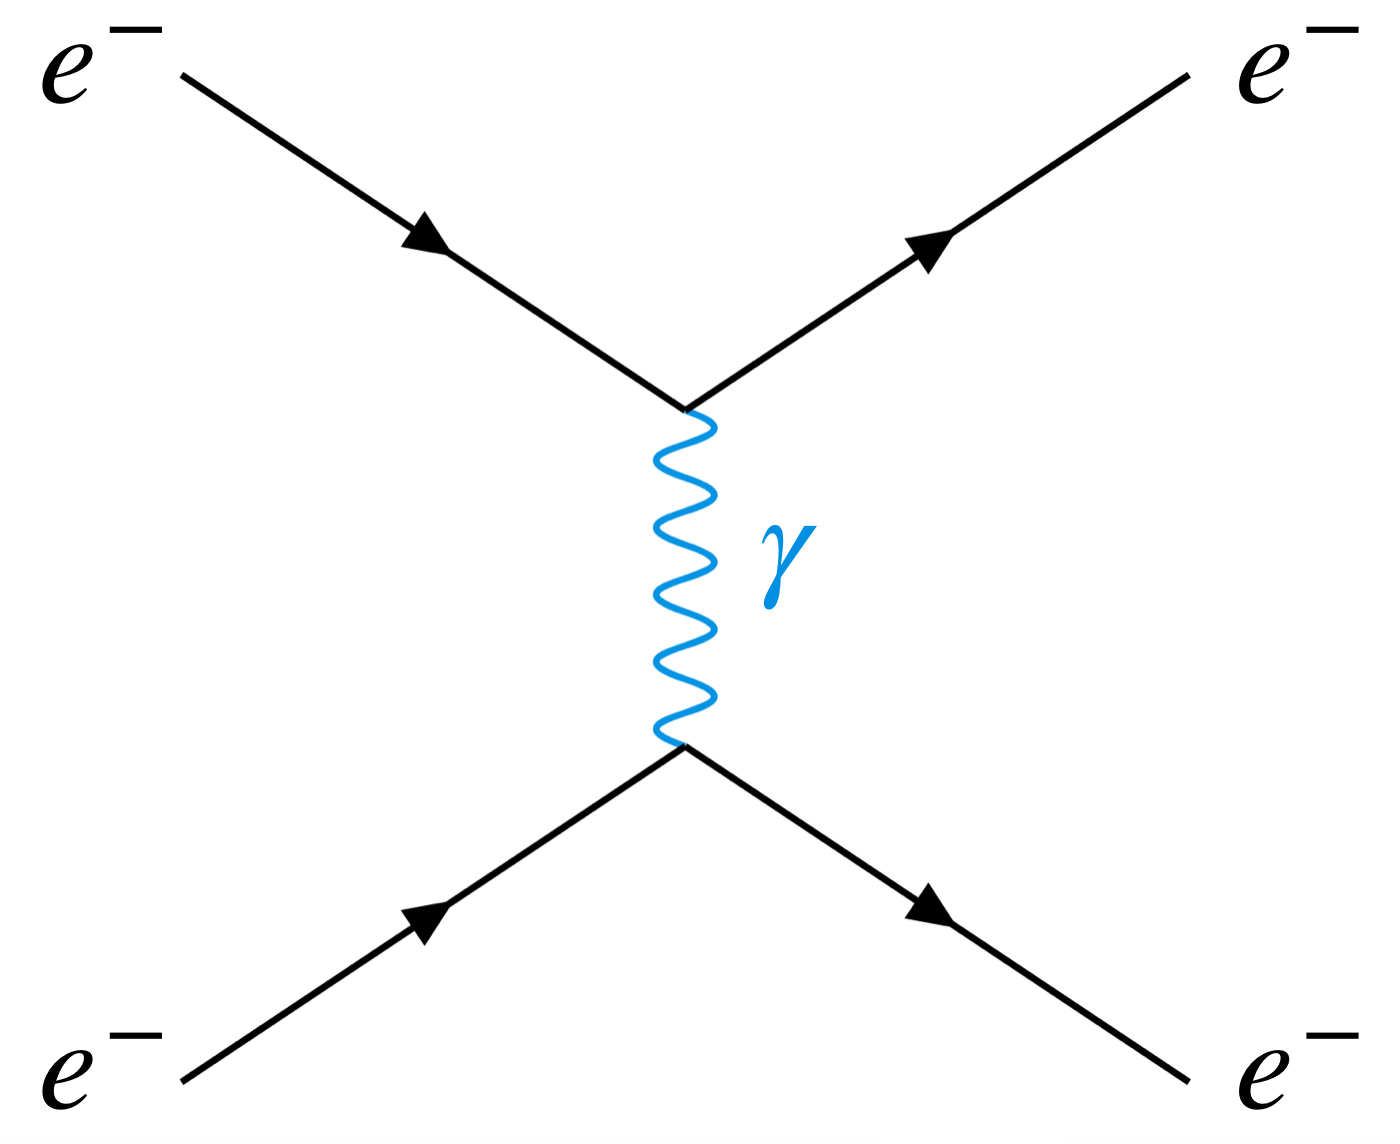
\includegraphics[width=6cm,height=6cm,keepaspectratio]{figures/sm/ee_scattering_moeller.png}
    \captionof{figure}
    \begin{tikzpicture}
        \begin{feynman}[large]
            \centering
            \vertex (h) {$h$}; % h at beginning 
            \vertex [right=1cm of h] (ZZ); % h -> ZZ vertex
            \node [circle, fill=black, inner sep=2pt, above right = 1cm and 1.25cm of ZZ] (Z1); % black dot node at epsilon (control size with ) 
            \node [above left = 7pt and 7pt of Z1] (e) {$\epsilon$}; % node with epsilon text
            \vertex [below right = 1cm and 2.5cm of ZZ] (Z2); % h -> ZZ bottom Z
            \vertex [above right = 0.5cm and 1.25cm of Z2] (Z2l1) {$l$}; % bottom Z -> ll (top l)
            \vertex [below right = 0.5cm and 1.25cm of Z2] (Z2l2) {$l$}; % bottom Z -> ll (bottom l)
            \vertex [above right = 1cm and 1.25cm of Z1] (ZD); % ZD
            \vertex [above right = 0.5cm and 1.25cm of ZD] (ZDl1) {$l$}; % ZD -> ll (top l)
            \vertex [below right = 0.5cm and 1.25cm of ZD] (ZDl2) {$l$}; % ZD -> ll (bottom l)
            \diagram* {
                (h) -- [scalar] (ZZ),
                (ZZ) -- [boson, edge label=$Z$] (Z1),
                (ZZ) -- [boson, edge label=$Z$] (Z2),
                (Z1) -- [boson, edge label=$Z_D$] (ZD),
                (ZDl2) -- [fermion] (ZD) -- [fermion] (ZDl1);
                (Z2l2) -- [fermion] (Z2) -- [fermion] (Z2l1);
            };
        \end{feynman}
    \end{tikzpicture}
        [Feynman diagram showing electron--electron (Møller) scattering]
        {Feynman diagram showing electron--electron (Møller) scattering.} 
    \label{fig:ee_scattering}
\end{multiFigure}
%%%%%%%%%%%%%%%%%%%%

\subsubsection{Bosons: Use the Force}

\emph{How do two electrons ``know'' that one is near the other and that they should repel?}
\Cref{fig:ee_scattering} shows a Feynman diagram of two electrons interacting with one other by means of an intermediate, virtual photon $(\gamma)$.
In QFT, mediator particles are called bosons---like the photon---convey interactions beween two interacting electrons.
The idea is that the photon carries momentum away from the first electron and carries it to the second one, therefore making it appear as if the two electrons are repelling one another.
The photon is not a measurable particle in this case, so it is said to be a \emph{virtual} photon.
This is why gauge bosons are often called the force carriers.

% Quantum Electrodynamics, one of the theories cooped up in the SM, is a quantum field theory that can mathematically describe one electron "throwing" a photon to the other.
The Feynman diagram in Fig.~\ref{fig:ee_scattering} is a simple way to visualize particle physics processes, although it must be stated that it does not depict what \emph{actually} happens between particles.
Feynman diagrams are instead a useful tool to help calculate the probabilities with which various processes happen.
Each diagram represents a single, scalar number that is calculated from a QFT integral and indicates how likely a process is to happen.
% Another benefit of Feynman Diagrams is their tinker-toy-like connectab you can string them together in novel ways to predict real-world processes.
Thus, QED is able to calculate the probability the electrons mediating such a photon between them. 
It's not just limited to electrons mediating photons, however.
The prediction capabilities of QED and other QFTs reach astounding accuracy how likely a process is to happen, between whichever particles and fields. 
One just needs to know the particle properties first.
% \emph{Any} particle with electric charge can interact via the electromagnetic force (EM) force.

Thus, the first force carrier---the first gauge boson---has been presented: the photon.
It is a massless particle and it is the mediator of the EM force. 
Photons only interact with particles that carry \emph{electric charge}.
The kind of charge that a particle carries ultimately determines with which bosons it may interact and via which forces.
The four fundamental forces found in nature are (in order of decreasing relative strength):
\begin{enumerate}
    \item strong force: $\mathcal{O}(1)$
    \item EM force: $\mathcal{O}(10^{-2})$
    \item weak force: $\mathcal{O}(10^{-13})$
    \item gravitational force: $\mathcal{O}(10^{-38})$
\end{enumerate}

\emph{If the photon mediates the EM force, then what mediates the other forces?}
The mediators of the strong force are the 8 gluons. 
Similar to the photon, they are also massless.
Gluons are trapped inside of protons, neutrons, and other hadronic matter. 
They `glue' nuclei to together, hence their name.
Just as photons only interact with particles that have electric charge, gluons only interact with particles that have \emph{color} charge.
There are three kinds of color charges---red, green, and blue---though not at all related to everyday visual color.
Each color has its corresponding anticolor charge---antired, antigreen, and antiblue---which negates the corresponding color charge, much like how a `$+1$' electric charge neutralizes a `$-1$' charge.
Not only would a red--antired (or green--antigreen or blue--antiblue) charge pair be considered a colorless (neutral) state but so too would the combination of red--green--blue (or antired--antigreen--antiblue).
A phenomenon known as \emph{color confinement} suggests that only colorless bound states are observable.
Interestingly, gluons themselves carry color charge (typically a color--anticolor combination) which they mediate between quarks (fermions discussed below).  % TODO: This may be repeated below.
This is in direct contrast to the photon which does not itself carry its associated charge (the electric charge).

There are three bosons which mediate the weak force: the \PZ, $\PW^+$, and $\PW^-$.
They are extraordinarily massive particles, weighing in at $91.2\GeV$ for the \PZ and $80.4\GeV$ for both kinds of \PW bosons. 
That means the W bosons has more mass than an iron atom!
These bosons interact with any particle that carries ``weak hypercharge'' ($Y_W$).
% The weak force has plagued physicists for nearly a century until only recently.
Particles which decay via the weak force live an astonishingly long time. 
Take for example the decay of a neutral pion into two photons:
$\pi^0 \to \gamma \gamma$. 
The decay occurs \emph{very} quickly---$\mathcal{O}(\tentotheminus{18}\snd)$---because it is mediated by the EM force.
Now consider the decay of a charged kaon into 3 charged pions:
$K^+ \to \pi^+ \pi^+ \pi^-$.
This decay occurs \emph{much} more slowly---$\mathcal{O}(\tentotheminus{8}\snd)$---compared to the $\pi^0$ decay.
The difference of over 10 orders of magnitude is because the charged kaon decayed via the weak force (in this example).

The final boson is the scalar Higgs boson and will be introduced in Sec.~\ref{sec:higgs_mech}.

% 1. There are 12 kinds fermions which are the matter particles and comprise all the matter that you see and feel
% 2. And in the other group there are 5 kinds of bosons, which are the force carriers and help fermions communicate with each other. 

\subsubsection{Fermions: Each One Matters}
There are 12 kinds of fermions, which are the matter particles of the Universe.
Fermions have half-integer spin, typically a value of $1/2$, and can be split into one of two groups, depending on if they interact with the strong force (quarks) or not (leptons).
First, the leptons are explored below, followed by the quarks.

\textbf{Leptons:}
% Ultimately all the matter we see, feel, and interact with daily is composed of fermions.
% Referring back to Fig.~\ref{fig:particular_table}, Fermions can be categorized into two groups: \textbf{leptons} and \textbf{quarks}.
One lepton was already introduced earlier: the electron (\Pe).
Looking again at the ``particular table'' (Fig.~\ref{fig:particular_table}), the electron has a ``cousin'' that is 200 times more massive than itself: the muon (\Pmu).
There is yet a lepton sibling even more massive than the \Pe or \Pmu: the tauon ($\tau$). 
All three of these leptons have the familiar $-1$ charge which allows them to interact via the EM force and exchange photons with other electrically charged particles.

The charged leptons also carry weak hypercharge, which allows them to interact via the weak force. 
If a charged lepton interacts with a \PWpm boson, it transforms into its corresponding ``partner''---the other member of the $SU(2)$ isospin doublet, the neutrino ($\nu$).
These fickle neutrinos \emph{only} interact via the weak force (and supposedly gravity) so they are effectively invisible, \ie very difficult to detect.
% They are very difficult to detect.

% How do we know that some particles, like protons and neutrons are actually composed of smaller bits, like these up and down quarks?
% Through deep inelastic scattering experiments, analogous to the Rutherford experiment,
% one can shoot electrons at these nucleons and probe into them.
% Thanks to the wave-particle duality of nature, these electrons can act like little wave bullets,
% that tunnel into the nucleon and sometimes... they bounce back. 

% For each charged lepton, it can transform it into its neutral form: 
% the corresponding neutrino. 
% For example, the muon can transform into a muon neutrino - and vice versa.
% To undergo this transformation, the muon must interact 
% with the appropriate boson: W-. 
% This conserves electric charge at this vertex.

% You can also view this diagram from another perspective 
% by rotating it. 
% Here we see a 

\textbf{Quarks:}
The six quarks are the fermions which interact with gluons.
They have \st{quarky} quirky names like: 
up, down, charm, strange, top, bottom. 
These are called the six ``flavors'' of quarks.
The top quark is an absolutely massive particle, being at the \emph{top} of the particle mass scale at $172.25^{+0.76}_{-0.77}\GeV$~\cite{Tumasyan:2779091}---approximately the same mass as a tungsten atom.

Quarks (\Pq) are electrically charged particles, but they have fractional charge.
Each quark in the top row of Fig.~\ref{fig:particular_table} has $+2/3$ electric charge and the bottom row has $-1/3$.
This is why combining two up quarks with a down quark to form a proton yields a net electric charge of $+1$.

Just as the leptons carried weak hypercharge and could interact via the weak force, so too can quarks. 
The $\PW^{\pm}$ bosons can change one flavor of quark into another.
The \PZ boson only affects the spin, momentum, and energy of the particle with which it interacts.

In addition to electric charge, quarks also carry one kind of color charge, which allows them to interact with gluons via the strong force. 
Quarks combine in different ways to form at least two types of hadrons.
The first (second) type of hadron is the \emph{baryon} (\emph{meson}), which is a particle that contains a combination of 3 (2) colorless quarks/antiquarks.
Examples of baryons are the familiar proton, consisting of the three-quark bound state $\Pqu \Pqu \Pqd$, and the neutron, consisting of the three-quark bound state $\Pqu \Pqd \Pqd$.
Examples of mesons are the pion $\pi^+$ $\left(\Pqu \Paqd \right)$\footnote{
    \textbf{Antiparticles:} Most particles have a corresponding \emph{antiparticle}, whose charges (\eg color charge, electric charge) are the opposite of the original particle's.
    Sometimes the notation for the antiparticle is obvious, like in the case of the electron $\left( \Pem \right)$ whose antiparticle is the positron $\left( \Pep \right)$.
    Other times, the common notation is to indicate an antiparticle with a \emph{bar} symbol over the letter, as is the case for a general quark (\Pq) and its corresponding antiquark $\left( \Paq \right)$
    Accounting for leptons, quarks, bosons, quark bound states, and now antiparticles, it's easy to see why it's called the ``\emph{particle zoo!}''
}, the kaon $K^-$ $\left(\Pqs \Paqu \right)$, and the $\jpsi$ $\left( \Pqc \Paqc \right)$.

\section{Mathematical Underpinnings of the SM}
\label{sec:sm_math}

Thanks to the brilliance of Professor Emmy Noether~\cite{Noether1918}, physics has greatly benefitted from the study of \emph{symmetry}.
She showed that the very existence of a symmetry \emph{implies} the conservation of an associated quantity (typically called a `current').
For example, if some law of physics is the same on Earth as it is on Mars (\eg $E = mc^2$ \emph{is} still true even across vast amounts of space), then there is an inherent symmetry (or ``sameness'') to the system across space and this \emph{implies} that the system obeys \emph{conservation of linear momentum}.
Similarly, if a system has rotational symmetry (\eg if you perform an experiment and get the same results facing north as you do facing southeast), then this \emph{implies} that the system obeys \emph{conservation of angular momentum}.
As a final---and astounding---example, a system that shows symmetry across time implies \emph{conservation of energy} within that system.

Particle physics makes use of \emph{gauge} symmetries, which lead to conservation of electric charge, color charge, \etc
By understanding such symmetries, the equations of motion (EOM) for a system are revealed (\ie how the system evolves throughout spacetime).
In particle physics, Newtonian mechanics is insufficient to obtain the EOM of quantum particles, so instead Lagrangian mechanics is used.
The first step is to write down the Euler--Lagrange equation~\cite{Halzen:1984mc}:
\begin{equation}
    % TODO: Use proper partial fractions commands from physics package.
    \frac{d}{\dt}
    \left( \frac{\partial \lagrang}{\partial \dot{q}_i} \right)
    -
    \frac{\partial \lagrang}{\partial q_i} = 0,
    \label{eqn:euler_lagrange}
\end{equation}
where the $q_i(t)$ are the time-dependent generalized coordinates of the associated particles
and \lagrang is the general Lagrangian function defined as:
\begin{equation*}
    \lagrang \equiv T - V,
\end{equation*}
where $T$ and $V$ are, respectively, the kinetic and potential energy functions of the system.
The second step is to find the stationary points using \cref{eqn:euler_lagrange} which yields the EOM of the system.

In particle physics, however, the generalized coordinates are promoted to particle \emph{wave functions}---functions of space and time:
\begin{align*}
    q_i(t) \to \phi(\vec{x}, t) & \equiv \phi(x_\mu)
    \\
    \lagrang(q_i, \dot{q}_i, t) \to  \lagrangdens & \left( \phi, \frac{\partial \phi}{\partial x_\mu}, x_\mu \right),
\end{align*}
where \lagrangdens is called the `Lagrangian density',
the idea being that at every point in space there is an associated value of \lagrang that still depends on time and the dynamical variables of the associated particles.
The Lagrangian density is related to \lagrang via:
\begin{equation*}
    \lagrang = \int{d^3x \, \lagrangdens}.
\end{equation*}
Gauge transformations can be applied to particle fields so long as \lagrangdens \emph{remains invariant}.

In all its glory, the SM Lagrangian density is given by~\cite{Halzen:1984mc, thesis_xunwu}:
\begin{align*}
    \lagrangdens =
    & - \frac{1}{4} B_{\mu \nu} B^{\mu \nu} - \frac{1}{4} W^a_{\mu \nu} W^{a \mu \nu} - \frac{1}{4} G^k_{\mu \nu} G^{k \mu \nu}
    \\
    & + \abs{D_\mu\Phi}^2 + \mu^2 \Phi^\dagger \Phi - \lambda \left( \Phi^\dagger \Phi \right)^2
    \\
    & + \sum_f{
        % \left[
            \bar{\psi}^f_R \left(i {\slashed D_\mu}\right) \psi_R^f + \bar{\psi}^f_L \left(i {\slashed D_\mu}\right) \psi_L^f
        % \right]
        }
    \\
    & + \sum_f{
        % \left[
            g_f \left[ \bar{\psi}_R^f \Phi^\dagger \psi_L^f + \bar{\psi}_L^f \Phi \psi_R^f + \bar{\psi}_R^f \tilde{\Phi}^\dagger \psi_L^f + \bar{\psi}_L^f \tilde{\Phi} \psi_R^f \right]
        % \right]
        },
\end{align*}
where the field strength tensors ($B_{\mu \nu}$, $W_{\mu \nu}^a$, $G_{\mu \nu}^k$) for their corresponding interaction fields
($B_\mu$, $W_\mu^a$, $G_\mu^k$)
of their associated symmetry groups are given by:
\begin{align*}
    U(1) : \quad & B_{\mu \nu}    = \partial_\mu B_\nu - \partial_\nu B_\mu
    \\
    SU(2) : \quad & W_{\mu \nu}^a  = \partial_\mu W_\nu^a - \partial_\nu W_\mu^a + g \varepsilon^{abc} W_\mu^b W_\nu^c
    \\
    SU(3) : \quad & G_{\mu \nu}^k  = \partial_\mu G_\nu^k - \partial_\nu G_\mu^k + g_s f^{klm} G_\mu^l G_\nu^m,
\end{align*}
where the slash notation is borrowed from \cref{eqn:dirac} and the gauge-transformed covariant derivative ($D_\mu$) is given by:
\begin{equation*}
    D_\mu = \partial_\mu - i g^\prime B_\mu Y - i g W_\mu^a T^a - i g_s G_\mu^k t^k,
\end{equation*}
where $g^\prime$ ($Y$), $g$ ($T^a$), and $g_s$ ($t^k$) are the field strength coefficients (interaction operators) for the $U(1)$, $SU(2)$, and $SU(3)$ groups, respectively,
and $\varepsilon^{abc}$ and $f^{klm}$ are the structure constants of the $SU(2)$ and $SU(3)$ groups which determine the group generators via:
\begin{align*}
     \left[ T^a, T^b \right] &= i \varepsilon^{abc} T_c
     \\
     \left[ t^k, t^l \right] &= i f^{klm} t_m
\end{align*}
% \Phi, \Phi^\dagger, \mu, \lambda,
% \psi_R^f, \bar{\psi}_R^f
where $a$ runs from 1--3 (from \cref{eqn:gamma_matrices}),
$k$ stands for the group generator indices and runs from 1--8,
% and finally the sums are taken over the fermion flavors $f$, and for each coupling there exists a coupling strength $g_f$.



% The main objective of the LHC is to probe the Electroweak Symmetry Breaking (EWSB) mechanism that generates the masses of the known elementary particles in the SM.
%  in the SMby the ATLAS~\cite{ATLAS:2012yve} and the CMS~\cite{CMS:2012qbp} collaborations and the subsequent studies of its properties with the full data set from Run 1, from 2009 to 2012, with a center-of-mass energy of 7\TeV and 8\TeV, provided the first opportunity to study this mechanism.
The discovery of the Higgs boson in 2012 confirmed the existence of the Higgs field, subsequently providing insight into the mechanism from which EWSB arises.
Not only does it explain the short-range nature of weak interactions but it also provides an explanation for the massive \PWpm and \PZ gauge bosons.

In the SM, the electroweak interactions are described by a gauge field theory invariant under the $SU(2)_L \times U(1)_Y$ symmetry group.
The mechanism of EWSB provides a general framework to preserve the structure of these gauge interactions at high energies~\cite{PhysRevD.2.1285, PhysRevLett.13.321, PhysRev.145.1156}.
The EWSB mechanism posits a self-interacting electroweak doublet of complex scalar fields, whose CP-even neutral component acquires a vacuum expectation value (VEV), which sets the scale of the symmetry breaking.
Four massless Goldstone bosons are generated, two of which linearly combine to give the \PWp and \PWm gauge bosons while the remaining two combine to give the photon $(\gamma)$ and the \PZ gauge bosons.
The masses of all fermions are also a consequence of EWSB since the Higgs field is postulated to couple to the fermions through Yukawa interactions.

\subsection{The Brout--Englert--Higgs Mechanism}
\label{sec:higgs_mech}

The SM lagrangian contains a scalar potential term that reads:
\begin{equation}
    V (\phi) = \mu^2\phi^\dagger\phi + \lambda(\phi^\dagger\phi)^2,
    \label{eqn:scalar_pot}
\end{equation}
where the Higgs field $\left( \phi(x) \right)$ is a self-interacting $SU(2)_L$ doublet of complex scalar fields containing 4 real degrees of freedom $\left( \phi^k \text{, where } k=1, 2, 3, 4 \right)$ with weak hypercharge $Y = 1$:
\begin{equation}
    \phi(x) = \frac{1}{\sqrt{2}}
    \begin{pmatrix}
        \sqrt{2}\phi^+ \\
        \phi^3 + i\phi^4
    \end{pmatrix},
    \label{eqn:higgs_doublet}
\end{equation}
where $\phi^3$ and $\phi^4$ are the CP-even and CP-odd neutral components, $\phi^+ \equiv \phi^1 + i \phi^2$ is the complex charged component of the Higgs doublet, and $V(\phi)$ is the most general renormalizable scalar potential.
The hypercharge is normalized such that $Q = T_{3} + \frac{Y}{2}$, where $Q$ is the electric charge and $T_{3}$ is the eigenvalue of the diagonal generator of $SU(2)_L$.

The case where $\lambda > 0$ in \cref{eqn:scalar_pot} indicates that a minimum exists in the potential and that $\phi$ is self-coupling~\cite{bass_higgs_2021}.
If $\mu^2 < 0$ is also required, then the minimum of $V(\phi)$ $\left( \ie \frac{\partial V}{\partial \phi} = 0 \right)$ occurs at:
\begin{equation}
    \abs{\phi} = \sqrt{ \frac{-\mu^2}{2\lambda} }.
    \label{eqn:higgs_min}
\end{equation}
% \begin{align*}
%     &\frac{\partial V}{\partial \phi} = 0
%     \\
%     \implies \abs{\phi} = &\sqrt{ \frac{-\mu^2}{2\lambda} }  \equiv \frac{v}{2},
% \end{align*}
This corresponds to the manifold of points that are invariant under the $SU(2)$ transformations~\cite{Halzen:1984mc}.
This ``Maxican hat'' potential is shown in \cref{fig:mex_hat} and illustrates the concept of spontaneous symmetry breaking.
%%%%%%%%%%%%%%%%%%%%
\begin{multiFigure}
    \centering
        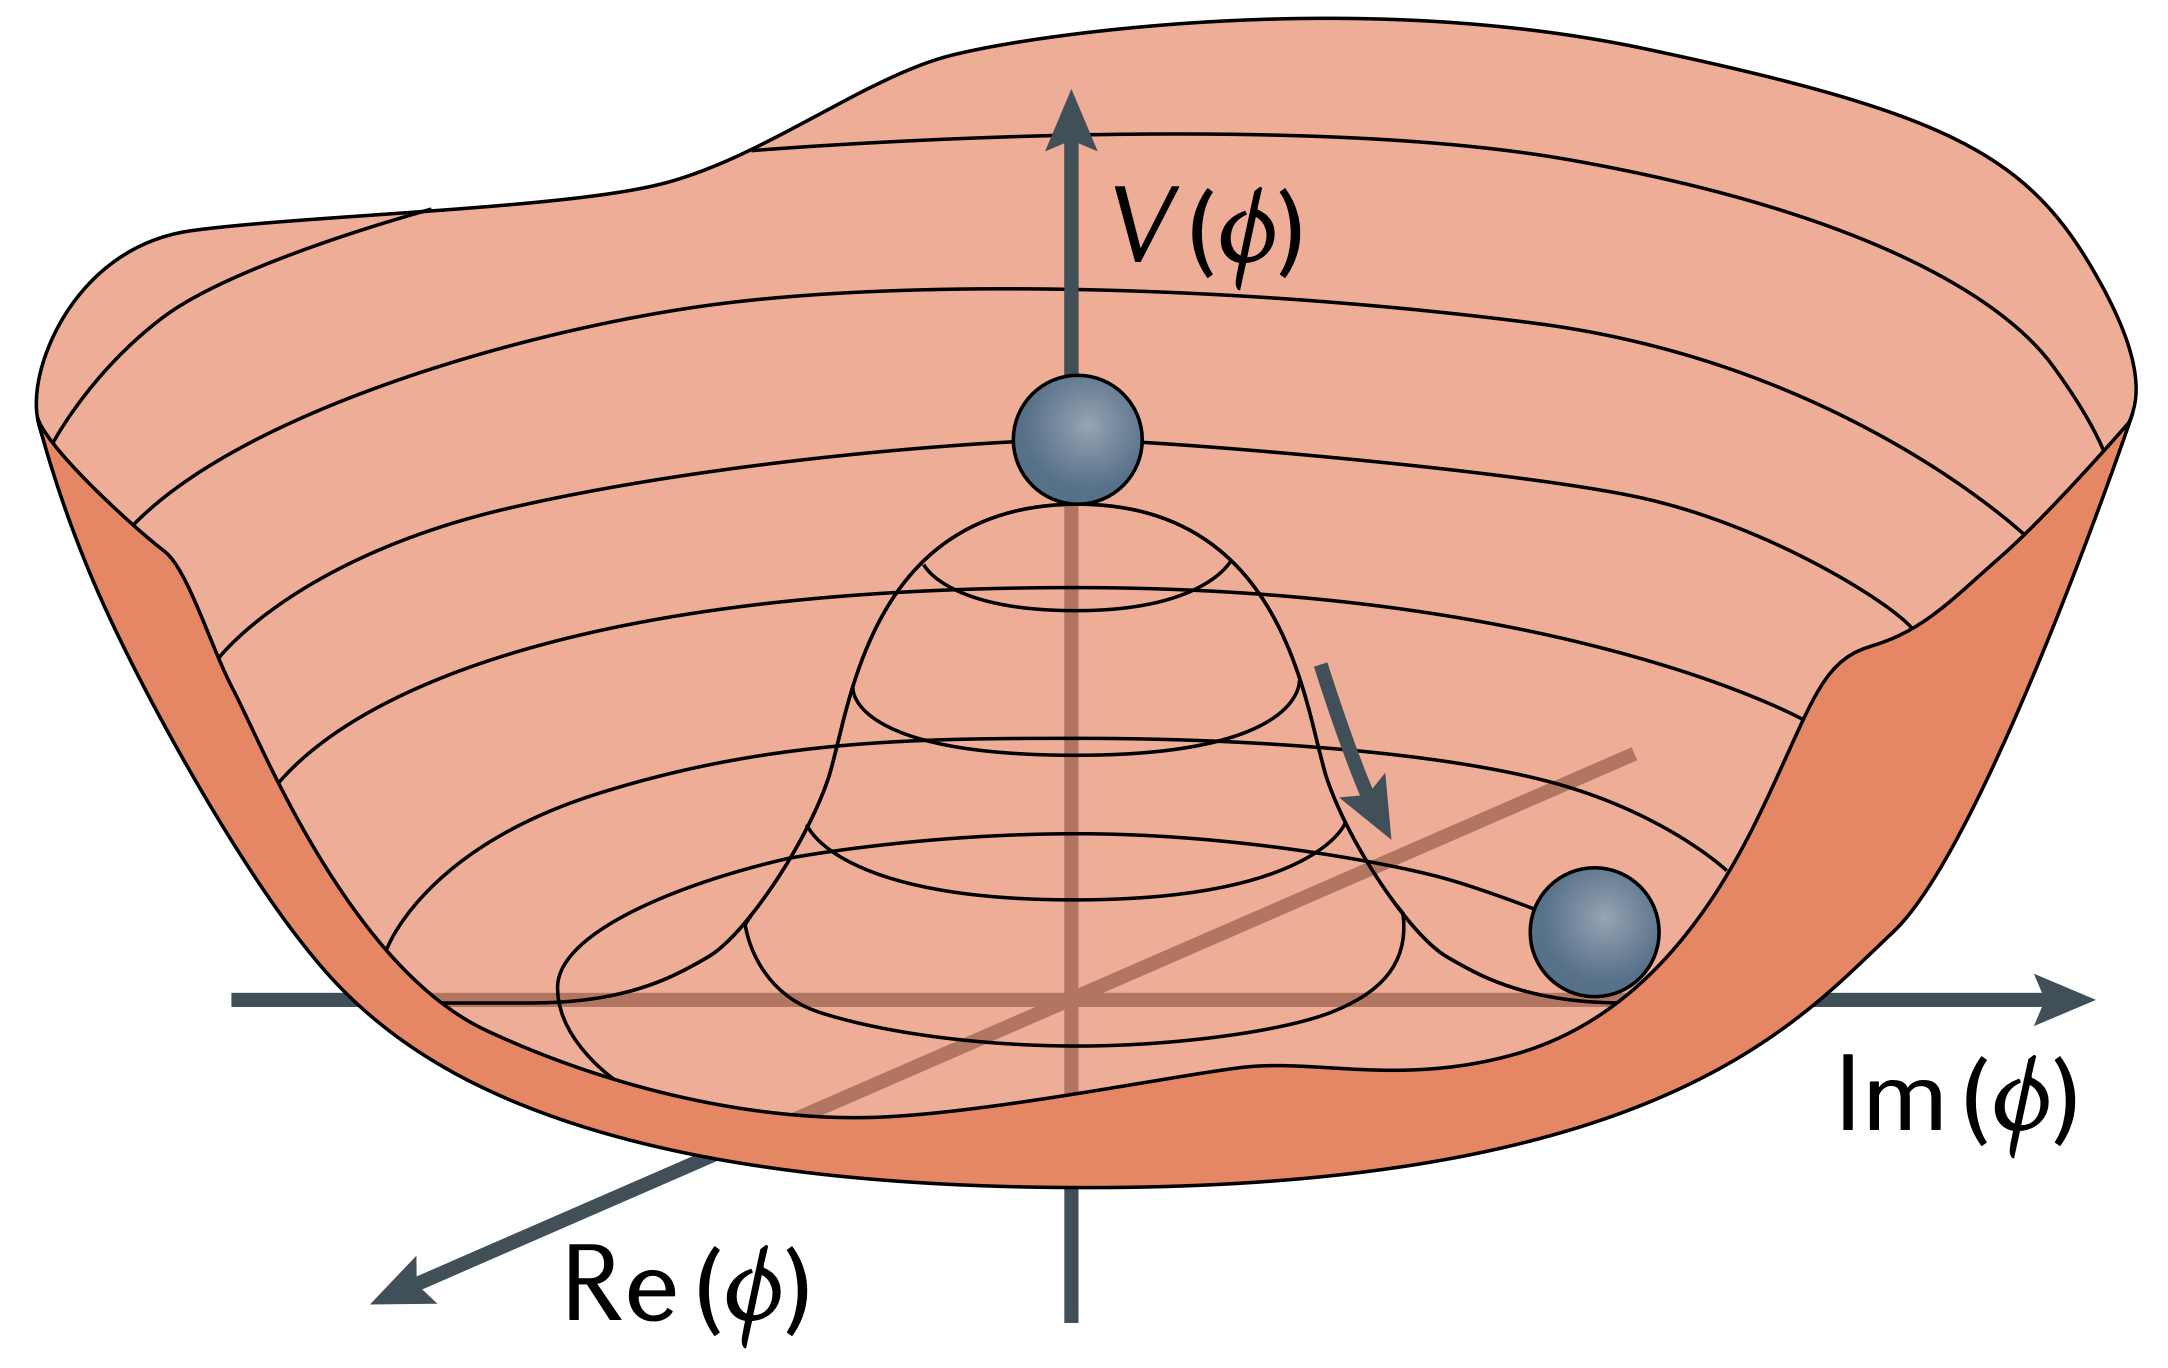
\includegraphics[height=6cm,keepaspectratio]{figures/sm/higgs_potential.png}
    \captionof{figure}
        [Mexican-hat-shaped Higgs potential for $\lambda > 0$ and $\mu^2 < 0$]
        {Mexican-hat-shaped Higgs potential for $\lambda > 0$ and $\mu^2 < 0$.
        Figure taken from~\cite{bass_higgs_2021}.} 
    \label{fig:mex_hat}
\end{multiFigure}
%%%%%%%%%%%%%%%%%%%%
Choosing the point $\phi^1 = \phi^2 = \phi^4 = 0$ in the manifold for convenience constrains $\left(\phi^3\right)^2 = \frac{-\mu^2}{\lambda} \equiv v^2$,
where $v$ is the Higgs VEV and has a value of 246\GeV. % TODO: Ref VEV value.
The doublet in Eqn.~\ref{eqn:higgs_doublet} can now be written as:
\begin{equation*}
    \langle\phi\rangle = \sqrt{\frac{1}{2}}
    \hspace{3pt}
    \begin{pmatrix}
        0 
        \\
        v 
    \end{pmatrix},
\end{equation*}
and expansion of $\phi(x)$ about this particular vacuum gives:
\begin{equation*}
    \phi(x) = 
    \sqrt{ \frac{1}{2} }
    \hspace{3pt}
    \begin{pmatrix}
        0
        \\
        v + H(x)
    \end{pmatrix},
\end{equation*}
where $H(x)$ is the scalar Higgs field.
Spontaneous breaking of the SM gauge symmetry $SU(3)_C \times SU(2)_L \times U(1)_Y$ into $SU(3)_C \times U(1)_\text{EM}$ has now been induced.

The global minimum of the theory defines the ground state, and spontaneous symmetry breaking implies that there is a global or local symmetry of the system that is not respected by the ground state.
From the four generators of the $SU(2)_L \times U(1)_Y$ SM gauge group, three are spontaneously broken, implying that they lead to non-trivial transformations of the ground state and indicate the existence of three massless Goldstone bosons identified with three of the four Higgs field degrees of freedom.
The Higgs field couples to the $W_\mu$ and $B_\mu$ gauge fields associated with the $SU(2)_L \times U(1)_Y$ local symmetry through the covariant derivative appearing in the kinetic term of the Higgs Lagrangian:
\begin{equation*}
    \lagrang_\text{Higgs} = (D_\mu\phi)^\dagger(D^\mu\phi) - V(\phi),
\end{equation*}
where $D_\mu\phi \equiv \left( \partial_\mu - ig \frac{\sigma^a}{2}W^a_\mu - ig^\prime \frac{Y}{2} B_\mu \right)\phi$,
and $\sigma^a$ (with $a = 1,2,3$) are the usual Pauli matrices,
and finally $g$ and $g^\prime$ are the $SU(2)_L$ and $U(1)_Y$ gauge couplings, respectively,
It is useful to note that:
\begin{equation*}
    \frac{g^\prime}{g} = \tan{\theta_W},
\end{equation*}
where $\theta_W$ is the weak mixing angle, which has been measured to be~\cite{noauthor_precision_2006}:
\begin{equation*}
    \sin^2{\theta_W} = 0.231\,53 \pm 0.000\,16,
\end{equation*}
though other measurements of $\theta_W$ have been performed~\cite{the_lhcb_collaboration_measurement_2015, cms_collaboration_measurement_2018}.
As a result, the neutral and the two charged massless Goldstone degrees of freedom mix with the gauge fields corresponding to the broken generators of $SU(2)_L$ and $U(1)_Y$:
\begin{align*}
    A_\mu &= B_\mu \cos{\theta_W}  + W^3_\mu \sin{\theta_W},
    \\
    Z_\mu &= -B_\mu \sin{\theta_W}  + W^3_\mu \cos{\theta_W},
\end{align*}
thus becoming, in the unitary gauge, the longitudinal components of the $\PZ$ and $\PW$ physical gauge bosons, respectively. % TODO: I don't think this is correct.
The $\PW$ and $\PZ$ gauge bosons acquire masses:
\begin{equation*}
    m_{\PW} = \frac{1}{2}vg, \hspace{7pt} m_{\PZ} = \frac{1}{2} v \sqrt{g^2+{g^\prime}^2},
\end{equation*}
from which the following relation is derived:
\begin{equation*}
    \frac{m_{\PW}}{m_{\PZ}} = \cos{\theta_W}.
\end{equation*}

The fourth generator remains unbroken since it is the one associated to the conserved $U(1)_\text{EM}$ gauge symmetry; thus, its corresponding gauge field---the photon ($\gamma$)---remains massless.
Similarly the eight color gauge bosons, the gluons ($g$), corresponding to the conserved $SU(3)_C$ gauge symmetry with 8 unbroken generators, also remain massless (though confined inside hadrons and mesons as the result of the asymptotic freedom behaviour of QCD).
Hence, from the initial four degrees of freedom of the Higgs field, two are absorbed by the $\PW^\pm$ gauge bosons, one by the $\PZ$ gauge boson, and the one remaining degree of freedom, $\PH$, is the physical Higgs boson---a relatively new and eponymous scalar particle dreamt of by Peter Higgs~\cite{PhysRevLett.13.321,PhysRev.145.1156}.
The Higgs boson is neutral under the electromagnetic interactions and transforms as a singlet under $SU(3)_C$ and hence does not couple at tree level to the massless photons and gluons.

The fermions of the SM acquire mass through renormalizable interactions between the Higgs field and the fermions, \ie the Yukawa interactions:
\begin{equation*}
    -\lagrang_\text{Yukawa} = \hat{h}^{(d)}_{ij} \bar{q}_{L_i} \phi d_{R_j} +
    \hat{h}^{(u)}_{ij} \bar{q}_{L_i} \tilde{\phi} u_{R_j} +
    \hat{h}^{(\ell)}_{ij} \bar{\ell}_{L_i} \phi e_{R_j} + h.c.,
\end{equation*}
which respect the symmetries of the SM but generate fermion masses once EWSB occurs.
The indices $i,j = 1,2,3$ refer to the three families of up quarks, down quarks, or charged leptons.
In the Lagrangian above, $\tilde{\phi} = i\sigma_2\phi^*$ while $q_L$ ($\ell_L$) and $u_R$, $d_R$ ($e_R$) are the quark (lepton) $SU(2)_L$ doublets and singlets, respectively, while in each term $\hat{h}^{(f)}_{{ij}}$ is parameterized by a $3\times3$ coupling matrix for the appropriate fermion ($f$).
% The mass term for neutrinos is omitted, but could be added in an analogous manner to the up-type quarks when right-handed neutrinos are supplementing the SM particle content (neutrinos can also acquire Majorana masses via non-renormalizable dimension-5 interactions with the Higgs field~\cite{Weinberg:1979sa}).
Once the Higgs field acquires a VEV, and after rotation to the fermion mass eigenstate basis that also diagonalizes the Higgs--fermion interactions, $\hat{h}^{(f)}_{ij} \rightarrow h^{(f)}_{i} \delta_{ij}$, all fermions acquire a mass given by:
\begin{equation*}
    m^{(f)}_{i} = \frac{h^{(f)}_{i} v}{\sqrt{2}}.
\end{equation*}
Finally, looking back at the first two terms of Eqn.~\ref{eqn:scalar_pot} reveals the mass of the SM Higgs boson $(\mH)$ in terms of the parameters $v$ and $\lambda$:
\begin{equation*}
    \mH = \sqrt{2 \lambda} v.
\end{equation*}
It should be noted that the EWSB mechanism provides no additional insight into possible underlying reasons for the large variety of masses of the fermions, often referred to as the \emph{flavor hierarchy}.
The fermion masses, accounting for a large number of the free parameters of the SM, are simply translated into Yukawa couplings.



% % At room temperature, we know that the weak force, which mediates decays of radioactive substances, is very different from the EM force.
% % However, at large energy scales, like those found during the Big Bang or those produced in the energetic proton--proton collisions of the Large Hadron Collider, the electromagnetic (EM) force and weak force are unified. 
% At large energy scales, like those found during the Big Bang or those produced in the energetic proton--proton collisions of the Large Hadron Collider, the electromagnetic (EM) force and weak nuclear force are one and the same: they are unified.
% However, at lower temperatures (like room temperature for example), we know that the weak force is very different from the EM force.
% The former mediates decays of radioactive substances, whereas the latter mediates the excitation of electrons in an atom.
% So what is responsible for the separation of these two forces, this so-called \emph{electroweak symmetry breaking}?

% Upon writing down the equations of motion from the SM Lagrangian (easier said than done), one discovers that all the particles mentioned earlier should have \emph{no mass}.
% Well that's a problem because most particles in nature definitely have mass, like the quarks, leptons, W$^{\pm}$, and Z bosons.
% % Since mass is a scalar, one can introduce a scalar field (spin 0) into the Lagrangian.
% By introducing a complex SU(2) doublet of scalar fields into the SM Lagrangian, in such a way that it leaves the Lagrangian invariant, then all peace can be restored.
% This scalar field turns out to be the Higgs field, and its excitations are Higgs bosons.
% Doing so reveals the particle which should have mass,
% The process of introducing a Higgs field and breaking the electroweak symmetry is called the \textbf{Higgs Mechanism}.

% % The Higgs field is required to be a scalar field and consists of a complex doublet, with four degrees of freedom.
% Each particle interacts with the Higgs field with a different strength: in fact, a particle's coupling strength to the Higgs field is exactly its mass! 
% The more the particle interacts with the Higgs field, the more mass it gains.
% Excitations, or quanta, of the Higgs field are Higgs bosons and are a direct consequence of introducing a Higgs scalar field into the SM Lagrangian to allow particles to have mass.


% \begin{itemize}
%     \item strong force $(1)$
%     \item EM force $(10^{-1})$
%     \item weak force $(10^{-13})$
%     \item gravitational force $(10^{-40})$
% \end{itemize}
% Speaking of forces, the four fundamental forces found in nature, along with their decreasing, relative strength are: 

% \textbf{Electroweak Interaction}
% Particles can interact with one another at long range.
% For example, an electron can emit a photon which can travel a 

% Electromagnetic force and weak force were unified Electroweak symmetry.
% This introduced 4 electroweak bosons: the photon, Z, W+, and W-.
% Then lectroweak symmetry breaking happened.
% This made the photon massless and the Z, W+, and W- as (very) massive.

% \textbf{Higgs Mechanism}
% Force field that fills space in the whole Universe but has no source or direction.
% The field has the same field at every point.
% It's a scalar field with spin 0.
% It does have electroweak charge.

\section{Shortcomings of the SM}
\label{sec:shortcomings}

More and more experimental measurements are being published that present results which significantly deviate from SM predictions.
One such measurement comes from the Collider Detector at Fermilab (CDF) Collaboration, which recently measured the mass of the \PW boson $(\mass{\PW})$ to be $80\,433.5 \pm 9.4\MeV$, whereas the SM predicts a mass of $80\,357 \pm 4\MeV$---a discrepancy of 7.0 standard deviations~\cite{cdf_collaboration_high-precision_2022}.
The CDF measurement of \mass{\PW}, along with measurements performed by other collaborations, is shown in Fig.~\ref{fig:wmass}.
%%%%%%%%%%%%%%%%%%%%
\begin{multiFigure}
    \centering
        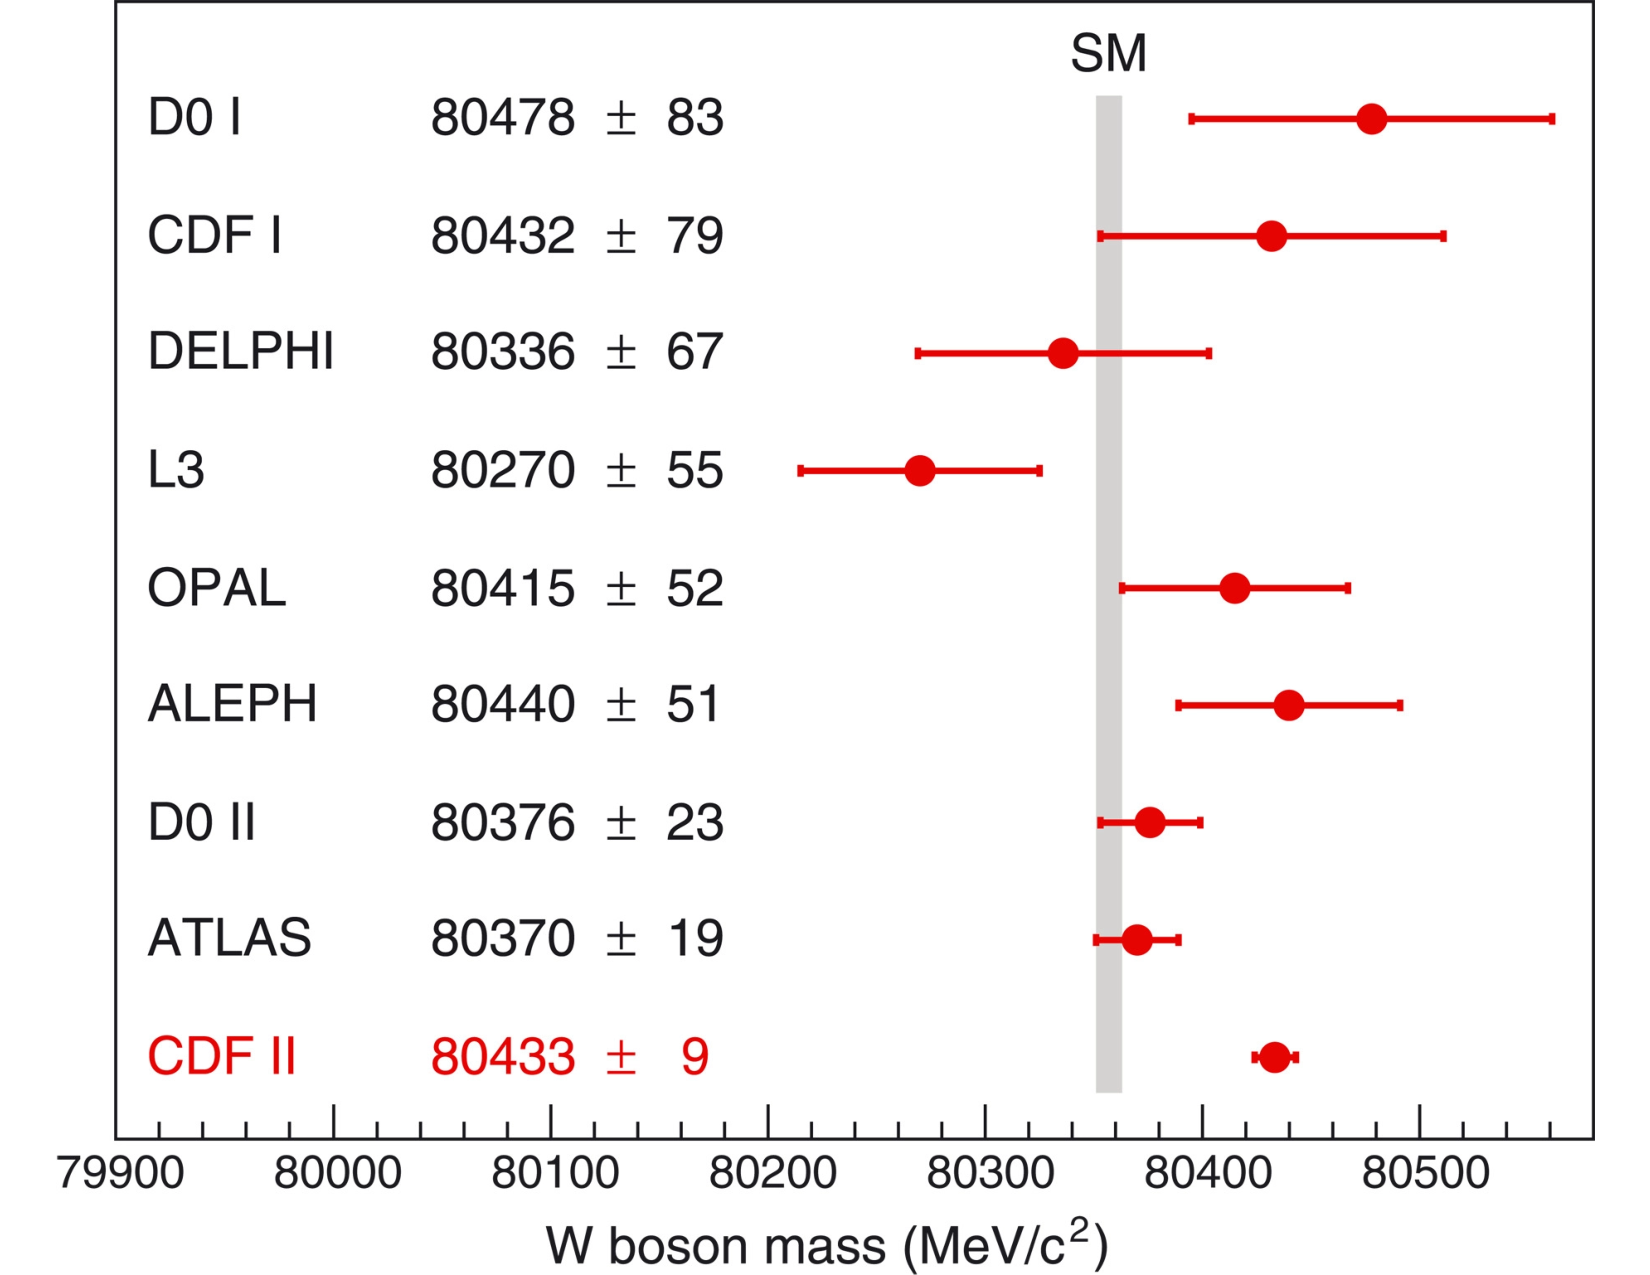
\includegraphics[height=8cm,keepaspectratio]{figures/sm/wmass.pdf}
    \captionof{figure}
        [Precision measurements of the \PW boson mass performed by various collaborations]
        {Precision measurements of the \PW boson mass performed by various collaborations.
        Plot taken from~\cite{cdf_collaboration_high-precision_2022}.} 
    \label{fig:wmass}
\end{multiFigure}
%%%%%%%%%%%%%%%%%%%%
Another recent result comes from the Baksan Experiment on Sterile Transitions, which suggests that electron neutrinos oscillate between sterile neutrino states~\cite{PhysRevLett.128.232501}.

Moreover, fermion masses are not predicted by the SM;
their masses are parameters of the theory and so must be experimentally measured~\cite{Halzen:1984mc}.
Additionally, the SM does not
\begin{itemize}
    \item \ldots incorporate gravity on a mathematical quantum level
    \item \ldots explain the matter/antimatter asymmetry of the Universe
    \item \ldots predict the existence of dark matter
    \item \ldots explain why there should be exactly three generations of fermions~\cite{particle_data_group_review_2020}.
\end{itemize}

Therefore, the foundation of the SM must continue to be scrutinized via particle collider experiments.
Hadrons are a reasonable choice for particle collisions, since hadronic matter is full of constituent parts---appropriately called \emph{partons}---like quarks and gluons.
By im\emph{part}ing immense amounts of energy into the partons and smashing them together, this allows the partons to interact and convert their energies into new kinds of matter.
One of the primary grounds of investigation to test the SM is at the world's largest circular particle collider: the Large Hadron Collider (Ch.~\ref{ch:lhc}).
